% Options for packages loaded elsewhere
\PassOptionsToPackage{unicode}{hyperref}
\PassOptionsToPackage{hyphens}{url}
%
\documentclass[
]{book}
\usepackage{amsmath,amssymb}
\usepackage{lmodern}
\usepackage{ifxetex,ifluatex}
\ifnum 0\ifxetex 1\fi\ifluatex 1\fi=0 % if pdftex
  \usepackage[T1]{fontenc}
  \usepackage[utf8]{inputenc}
  \usepackage{textcomp} % provide euro and other symbols
\else % if luatex or xetex
  \usepackage{unicode-math}
  \defaultfontfeatures{Scale=MatchLowercase}
  \defaultfontfeatures[\rmfamily]{Ligatures=TeX,Scale=1}
\fi
% Use upquote if available, for straight quotes in verbatim environments
\IfFileExists{upquote.sty}{\usepackage{upquote}}{}
\IfFileExists{microtype.sty}{% use microtype if available
  \usepackage[]{microtype}
  \UseMicrotypeSet[protrusion]{basicmath} % disable protrusion for tt fonts
}{}
\makeatletter
\@ifundefined{KOMAClassName}{% if non-KOMA class
  \IfFileExists{parskip.sty}{%
    \usepackage{parskip}
  }{% else
    \setlength{\parindent}{0pt}
    \setlength{\parskip}{6pt plus 2pt minus 1pt}}
}{% if KOMA class
  \KOMAoptions{parskip=half}}
\makeatother
\usepackage{xcolor}
\IfFileExists{xurl.sty}{\usepackage{xurl}}{} % add URL line breaks if available
\IfFileExists{bookmark.sty}{\usepackage{bookmark}}{\usepackage{hyperref}}
\hypersetup{
  pdftitle={Statistics Tips},
  pdfauthor={Øystein Sørensen},
  hidelinks,
  pdfcreator={LaTeX via pandoc}}
\urlstyle{same} % disable monospaced font for URLs
\usepackage{color}
\usepackage{fancyvrb}
\newcommand{\VerbBar}{|}
\newcommand{\VERB}{\Verb[commandchars=\\\{\}]}
\DefineVerbatimEnvironment{Highlighting}{Verbatim}{commandchars=\\\{\}}
% Add ',fontsize=\small' for more characters per line
\usepackage{framed}
\definecolor{shadecolor}{RGB}{248,248,248}
\newenvironment{Shaded}{\begin{snugshade}}{\end{snugshade}}
\newcommand{\AlertTok}[1]{\textcolor[rgb]{0.94,0.16,0.16}{#1}}
\newcommand{\AnnotationTok}[1]{\textcolor[rgb]{0.56,0.35,0.01}{\textbf{\textit{#1}}}}
\newcommand{\AttributeTok}[1]{\textcolor[rgb]{0.77,0.63,0.00}{#1}}
\newcommand{\BaseNTok}[1]{\textcolor[rgb]{0.00,0.00,0.81}{#1}}
\newcommand{\BuiltInTok}[1]{#1}
\newcommand{\CharTok}[1]{\textcolor[rgb]{0.31,0.60,0.02}{#1}}
\newcommand{\CommentTok}[1]{\textcolor[rgb]{0.56,0.35,0.01}{\textit{#1}}}
\newcommand{\CommentVarTok}[1]{\textcolor[rgb]{0.56,0.35,0.01}{\textbf{\textit{#1}}}}
\newcommand{\ConstantTok}[1]{\textcolor[rgb]{0.00,0.00,0.00}{#1}}
\newcommand{\ControlFlowTok}[1]{\textcolor[rgb]{0.13,0.29,0.53}{\textbf{#1}}}
\newcommand{\DataTypeTok}[1]{\textcolor[rgb]{0.13,0.29,0.53}{#1}}
\newcommand{\DecValTok}[1]{\textcolor[rgb]{0.00,0.00,0.81}{#1}}
\newcommand{\DocumentationTok}[1]{\textcolor[rgb]{0.56,0.35,0.01}{\textbf{\textit{#1}}}}
\newcommand{\ErrorTok}[1]{\textcolor[rgb]{0.64,0.00,0.00}{\textbf{#1}}}
\newcommand{\ExtensionTok}[1]{#1}
\newcommand{\FloatTok}[1]{\textcolor[rgb]{0.00,0.00,0.81}{#1}}
\newcommand{\FunctionTok}[1]{\textcolor[rgb]{0.00,0.00,0.00}{#1}}
\newcommand{\ImportTok}[1]{#1}
\newcommand{\InformationTok}[1]{\textcolor[rgb]{0.56,0.35,0.01}{\textbf{\textit{#1}}}}
\newcommand{\KeywordTok}[1]{\textcolor[rgb]{0.13,0.29,0.53}{\textbf{#1}}}
\newcommand{\NormalTok}[1]{#1}
\newcommand{\OperatorTok}[1]{\textcolor[rgb]{0.81,0.36,0.00}{\textbf{#1}}}
\newcommand{\OtherTok}[1]{\textcolor[rgb]{0.56,0.35,0.01}{#1}}
\newcommand{\PreprocessorTok}[1]{\textcolor[rgb]{0.56,0.35,0.01}{\textit{#1}}}
\newcommand{\RegionMarkerTok}[1]{#1}
\newcommand{\SpecialCharTok}[1]{\textcolor[rgb]{0.00,0.00,0.00}{#1}}
\newcommand{\SpecialStringTok}[1]{\textcolor[rgb]{0.31,0.60,0.02}{#1}}
\newcommand{\StringTok}[1]{\textcolor[rgb]{0.31,0.60,0.02}{#1}}
\newcommand{\VariableTok}[1]{\textcolor[rgb]{0.00,0.00,0.00}{#1}}
\newcommand{\VerbatimStringTok}[1]{\textcolor[rgb]{0.31,0.60,0.02}{#1}}
\newcommand{\WarningTok}[1]{\textcolor[rgb]{0.56,0.35,0.01}{\textbf{\textit{#1}}}}
\usepackage{longtable,booktabs,array}
\usepackage{calc} % for calculating minipage widths
% Correct order of tables after \paragraph or \subparagraph
\usepackage{etoolbox}
\makeatletter
\patchcmd\longtable{\par}{\if@noskipsec\mbox{}\fi\par}{}{}
\makeatother
% Allow footnotes in longtable head/foot
\IfFileExists{footnotehyper.sty}{\usepackage{footnotehyper}}{\usepackage{footnote}}
\makesavenoteenv{longtable}
\usepackage{graphicx}
\makeatletter
\def\maxwidth{\ifdim\Gin@nat@width>\linewidth\linewidth\else\Gin@nat@width\fi}
\def\maxheight{\ifdim\Gin@nat@height>\textheight\textheight\else\Gin@nat@height\fi}
\makeatother
% Scale images if necessary, so that they will not overflow the page
% margins by default, and it is still possible to overwrite the defaults
% using explicit options in \includegraphics[width, height, ...]{}
\setkeys{Gin}{width=\maxwidth,height=\maxheight,keepaspectratio}
% Set default figure placement to htbp
\makeatletter
\def\fps@figure{htbp}
\makeatother
\setlength{\emergencystretch}{3em} % prevent overfull lines
\providecommand{\tightlist}{%
  \setlength{\itemsep}{0pt}\setlength{\parskip}{0pt}}
\setcounter{secnumdepth}{5}
\usepackage{booktabs}
\ifluatex
  \usepackage{selnolig}  % disable illegal ligatures
\fi
\usepackage[]{natbib}
\bibliographystyle{plainnat}

\title{Statistics Tips}
\author{Øystein Sørensen}
\date{2022-01-27}

\begin{document}
\maketitle

{
\setcounter{tocdepth}{1}
\tableofcontents
}
\hypertarget{about}{%
\chapter{About}\label{about}}

This book is intended to be an ever-growing repository of statistics tips and tricks for the \href{https://www.oslobrains.no/}{Center for Lifespan Changes in Brain and Cognition}. I may not be able to add appropriate references everywhere, but in general the books \citet{wood2017a} and \citet{pinheiro2000} have been particularly useful for my own understanding.

\hypertarget{generalized-additive-mixed-models}{%
\chapter{Generalized Additive Mixed Models}\label{generalized-additive-mixed-models}}

\begin{Shaded}
\begin{Highlighting}[]
\FunctionTok{library}\NormalTok{(tidyverse)}
\end{Highlighting}
\end{Shaded}

\begin{verbatim}
## -- Attaching packages --------------------------------------- tidyverse 1.3.1 --
\end{verbatim}

\begin{verbatim}
## v ggplot2 3.3.5     v purrr   0.3.4
## v tibble  3.1.6     v dplyr   1.0.7
## v tidyr   1.1.4     v stringr 1.4.0
## v readr   2.1.1     v forcats 0.5.1
\end{verbatim}

\begin{verbatim}
## -- Conflicts ------------------------------------------ tidyverse_conflicts() --
## x dplyr::filter() masks stats::filter()
## x dplyr::lag()    masks stats::lag()
\end{verbatim}

\begin{Shaded}
\begin{Highlighting}[]
\FunctionTok{theme\_set}\NormalTok{(}\FunctionTok{theme\_bw}\NormalTok{())}
\FunctionTok{library}\NormalTok{(mgcv)}
\end{Highlighting}
\end{Shaded}

\begin{verbatim}
## Loading required package: nlme
\end{verbatim}

\begin{verbatim}
## 
## Attaching package: 'nlme'
\end{verbatim}

\begin{verbatim}
## The following object is masked from 'package:dplyr':
## 
##     collapse
\end{verbatim}

\begin{verbatim}
## This is mgcv 1.8-38. For overview type 'help("mgcv-package")'.
\end{verbatim}

The utility of GAMMs for estimating lifespan brain trajectories is described in \citet{fjell2010} and \citet{sorensen2021}. The main R packages for GAMMs are \texttt{mgcv} and \texttt{gamm4}.

\hypertarget{scannerbatch-effects}{%
\section{Scanner/batch effects}\label{scannerbatch-effects}}

A common problem is that longitudinal data have been collected on different scanners. There can be systematic differences between values estimated on different scanners, and they can have different noise levels. We will simulate some data to illustrate the problem.

\begin{Shaded}
\begin{Highlighting}[]
\NormalTok{scanners }\OtherTok{\textless{}{-}}\NormalTok{ letters[}\DecValTok{1}\SpecialCharTok{:}\DecValTok{4}\NormalTok{]}
\NormalTok{scanner\_bias }\OtherTok{\textless{}{-}} \FunctionTok{c}\NormalTok{(}\DecValTok{0}\NormalTok{, }\DecValTok{1}\NormalTok{, .}\DecValTok{4}\NormalTok{, .}\DecValTok{2}\NormalTok{)}
\NormalTok{scanner\_noise }\OtherTok{\textless{}{-}} \FunctionTok{c}\NormalTok{(}\DecValTok{1}\NormalTok{, }\DecValTok{1}\NormalTok{, }\DecValTok{2}\NormalTok{, .}\DecValTok{5}\NormalTok{)}
\FunctionTok{names}\NormalTok{(scanner\_bias) }\OtherTok{\textless{}{-}} \FunctionTok{names}\NormalTok{(scanner\_noise) }\OtherTok{\textless{}{-}}\NormalTok{ scanners}
\NormalTok{n }\OtherTok{\textless{}{-}} \DecValTok{1000}

\FunctionTok{set.seed}\NormalTok{(}\DecValTok{9988}\NormalTok{)}
\NormalTok{dat }\OtherTok{\textless{}{-}} \FunctionTok{tibble}\NormalTok{(}
  \AttributeTok{id =} \FunctionTok{seq\_len}\NormalTok{(n), }
  \AttributeTok{time =} \DecValTok{0}\NormalTok{,}
  \AttributeTok{random\_intercept =} \FunctionTok{rnorm}\NormalTok{(n)}
\NormalTok{  ) }\SpecialCharTok{\%\textgreater{}\%} 
  \FunctionTok{mutate}\NormalTok{(}\AttributeTok{num\_observations =} \FunctionTok{sample}\NormalTok{(}\DecValTok{1}\SpecialCharTok{:}\DecValTok{3}\NormalTok{, }\AttributeTok{size =} \FunctionTok{nrow}\NormalTok{(.), }\AttributeTok{replace =} \ConstantTok{TRUE}\NormalTok{)) }\SpecialCharTok{\%\textgreater{}\%} 
  \FunctionTok{uncount}\NormalTok{(num\_observations) }\SpecialCharTok{\%\textgreater{}\%} 
  \FunctionTok{group\_by}\NormalTok{(id) }\SpecialCharTok{\%\textgreater{}\%} 
  \FunctionTok{mutate}\NormalTok{(}\AttributeTok{timepoint =} \FunctionTok{row\_number}\NormalTok{()) }\SpecialCharTok{\%\textgreater{}\%} 
  \FunctionTok{ungroup}\NormalTok{() }\SpecialCharTok{\%\textgreater{}\%} 
  \FunctionTok{mutate}\NormalTok{(}
    \AttributeTok{time =} \FunctionTok{if\_else}\NormalTok{(timepoint }\SpecialCharTok{==} \DecValTok{1}\NormalTok{, time, }\FunctionTok{runif}\NormalTok{(}\FunctionTok{nrow}\NormalTok{(.), }\AttributeTok{max =}\NormalTok{ .}\DecValTok{5}\NormalTok{)),}
    \AttributeTok{scanner =} \FunctionTok{factor}\NormalTok{(}\FunctionTok{sample}\NormalTok{(scanners, }\AttributeTok{size =} \FunctionTok{nrow}\NormalTok{(.), }\AttributeTok{replace =} \ConstantTok{TRUE}\NormalTok{))}
\NormalTok{    ) }\SpecialCharTok{\%\textgreater{}\%} 
  \FunctionTok{group\_by}\NormalTok{(id) }\SpecialCharTok{\%\textgreater{}\%} 
  \FunctionTok{mutate}\NormalTok{(}\AttributeTok{time =} \FunctionTok{cumsum}\NormalTok{(time)) }\SpecialCharTok{\%\textgreater{}\%} 
  \FunctionTok{ungroup}\NormalTok{() }\SpecialCharTok{\%\textgreater{}\%} 
  \FunctionTok{mutate}\NormalTok{(}
    \AttributeTok{noise =} \FunctionTok{rnorm}\NormalTok{(}\FunctionTok{nrow}\NormalTok{(.), }\AttributeTok{sd =}\NormalTok{ scanner\_noise[scanner]),}
    \AttributeTok{bias =}\NormalTok{ scanner\_bias[scanner],}
    \AttributeTok{y =} \FloatTok{0.2} \SpecialCharTok{*}\NormalTok{ time}\SpecialCharTok{\^{}}\DecValTok{11} \SpecialCharTok{*}\NormalTok{ (}\DecValTok{10} \SpecialCharTok{*}\NormalTok{ (}\DecValTok{1} \SpecialCharTok{{-}}\NormalTok{ time))}\SpecialCharTok{\^{}}\DecValTok{6} \SpecialCharTok{+} \DecValTok{10} \SpecialCharTok{*} 
\NormalTok{      (}\DecValTok{10} \SpecialCharTok{*}\NormalTok{ time)}\SpecialCharTok{\^{}}\DecValTok{3} \SpecialCharTok{*}\NormalTok{ (}\DecValTok{1} \SpecialCharTok{{-}}\NormalTok{ time)}\SpecialCharTok{\^{}}\DecValTok{10} \SpecialCharTok{+}\NormalTok{ bias }\SpecialCharTok{+}\NormalTok{ noise }\SpecialCharTok{+}\NormalTok{ random\_intercept}
\NormalTok{  ) }\SpecialCharTok{\%\textgreater{}\%} 
  \FunctionTok{select}\NormalTok{(}\SpecialCharTok{{-}}\NormalTok{noise, }\SpecialCharTok{{-}}\NormalTok{bias, }\SpecialCharTok{{-}}\NormalTok{timepoint)}
\end{Highlighting}
\end{Shaded}

Here is a spaghetti plot of the data.

\begin{Shaded}
\begin{Highlighting}[]
\FunctionTok{ggplot}\NormalTok{(dat, }\FunctionTok{aes}\NormalTok{(}\AttributeTok{x =}\NormalTok{ time, }\AttributeTok{y =}\NormalTok{ y, }\AttributeTok{group =}\NormalTok{ id)) }\SpecialCharTok{+} 
  \FunctionTok{geom\_line}\NormalTok{(}\AttributeTok{alpha =}\NormalTok{ .}\DecValTok{3}\NormalTok{) }\SpecialCharTok{+} 
  \FunctionTok{geom\_point}\NormalTok{(}\FunctionTok{aes}\NormalTok{(}\AttributeTok{color =}\NormalTok{ scanner))}
\end{Highlighting}
\end{Shaded}

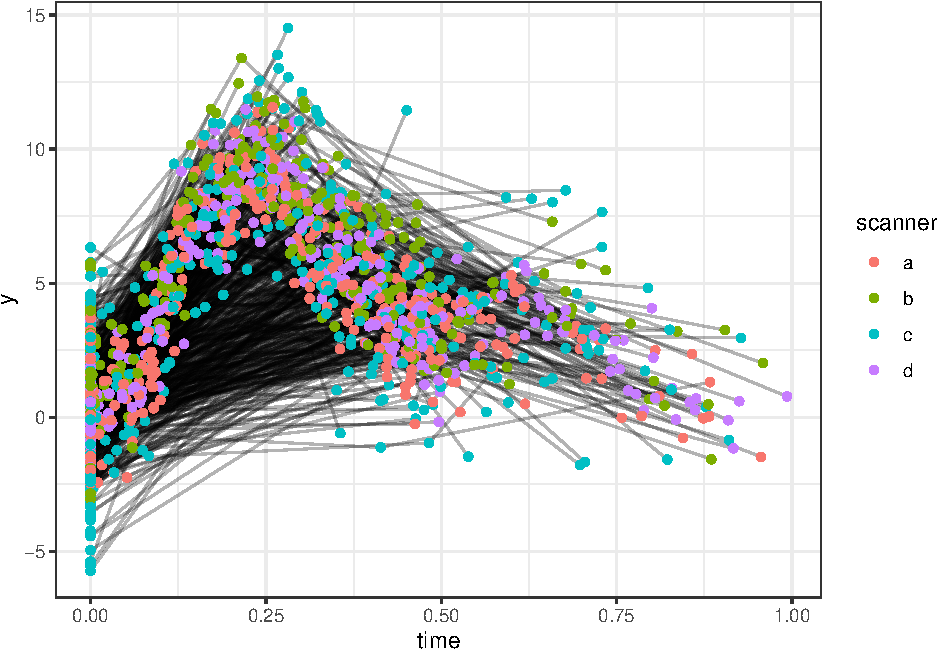
\includegraphics{_main_files/figure-latex/unnamed-chunk-4-1.pdf}

There are two ways of correcting for scanner bias. We can either include scanner as a fixed effect, or we can include it as a random effect. With as few as 4 scanners this will not make much of a difference in practice, but the interpretations of the models are a bit difference. With \emph{fixed effects} we are interested in the specific scanners in this study, and want to estimater \emph{their} bias. With \emph{random effects} we would consider scanners as samples from some population of scanners, and our interest would be in the variation between scanners. Given the limited number of scanners, we use fixed effects in this example.

\begin{Shaded}
\begin{Highlighting}[]
\NormalTok{mod1 }\OtherTok{\textless{}{-}} \FunctionTok{gamm}\NormalTok{(y }\SpecialCharTok{\textasciitilde{}} \FunctionTok{s}\NormalTok{(time) }\SpecialCharTok{+}\NormalTok{ scanner, }\AttributeTok{random =} \FunctionTok{list}\NormalTok{(}\AttributeTok{id =}\SpecialCharTok{\textasciitilde{}} \DecValTok{1}\NormalTok{), }\AttributeTok{data =}\NormalTok{ dat)}
\end{Highlighting}
\end{Shaded}

We can plot the model fit.

\begin{Shaded}
\begin{Highlighting}[]
\FunctionTok{plot}\NormalTok{(mod1}\SpecialCharTok{$}\NormalTok{gam)}
\end{Highlighting}
\end{Shaded}

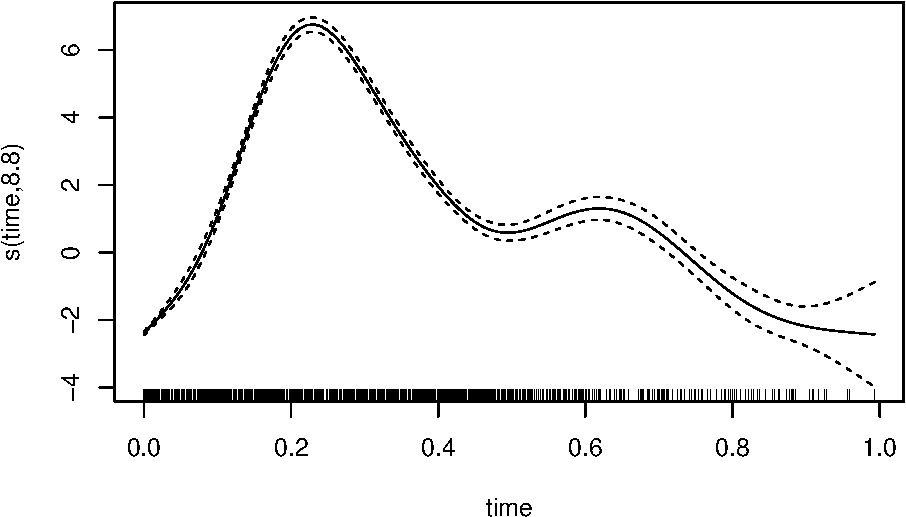
\includegraphics{_main_files/figure-latex/unnamed-chunk-6-1.pdf}

And inspect the output. We that the \texttt{scanner} term has discovered that there are systematic differences between the scanners. It won't be exact, since this is a randoom sample, but it points in the right directions.

\begin{Shaded}
\begin{Highlighting}[]
\FunctionTok{summary}\NormalTok{(mod1}\SpecialCharTok{$}\NormalTok{gam)}
\end{Highlighting}
\end{Shaded}

\begin{verbatim}
## 
## Family: gaussian 
## Link function: identity 
## 
## Formula:
## y ~ s(time) + scanner
## 
## Parametric coefficients:
##             Estimate Std. Error t value Pr(>|t|)    
## (Intercept)  2.36789    0.07091  33.392   <2e-16 ***
## scannerb     0.98792    0.09460  10.443   <2e-16 ***
## scannerc     0.14460    0.09211   1.570   0.1166    
## scannerd     0.16303    0.09376   1.739   0.0822 .  
## ---
## Signif. codes:  0 '***' 0.001 '**' 0.01 '*' 0.05 '.' 0.1 ' ' 1
## 
## Approximate significance of smooth terms:
##           edf Ref.df    F p-value    
## s(time) 8.795  8.795 1100  <2e-16 ***
## ---
## Signif. codes:  0 '***' 0.001 '**' 0.01 '*' 0.05 '.' 0.1 ' ' 1
## 
## R-sq.(adj) =  0.775   
##   Scale est. = 1.6241    n = 2026
\end{verbatim}

The model does however assume identical residuals, regardless of scanner. We can produce a diagnostic plot showing the residuals by scanner, which shows that this assumption is not correct (as we already new). In particular, scanner d has much lower residuals than scanner c.

\begin{Shaded}
\begin{Highlighting}[]
\FunctionTok{plot}\NormalTok{(mod1}\SpecialCharTok{$}\NormalTok{lme, }\AttributeTok{form =} \FunctionTok{resid}\NormalTok{(.) }\SpecialCharTok{\textasciitilde{}} \FunctionTok{fitted}\NormalTok{(.) }\SpecialCharTok{|}\NormalTok{ scanner)}
\end{Highlighting}
\end{Shaded}

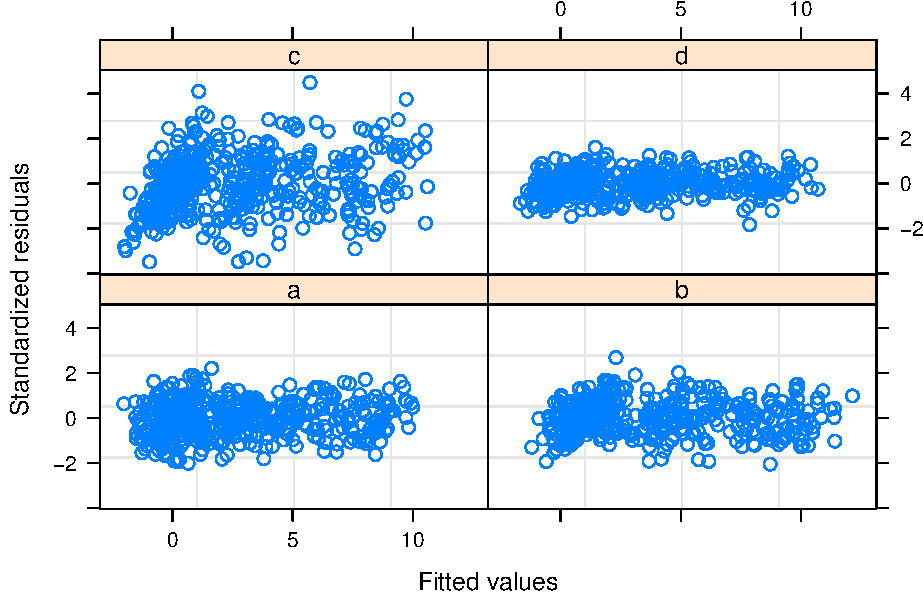
\includegraphics{_main_files/figure-latex/unnamed-chunk-8-1.pdf}

We can allow the residual standard deviation to differ between scanners.

\begin{Shaded}
\begin{Highlighting}[]
\NormalTok{mod2 }\OtherTok{\textless{}{-}} \FunctionTok{gamm}\NormalTok{(y }\SpecialCharTok{\textasciitilde{}} \FunctionTok{s}\NormalTok{(time) }\SpecialCharTok{+}\NormalTok{ scanner, }\AttributeTok{random =} \FunctionTok{list}\NormalTok{(}\AttributeTok{id =}\SpecialCharTok{\textasciitilde{}} \DecValTok{1}\NormalTok{), }
             \AttributeTok{weights =} \FunctionTok{varIdent}\NormalTok{(}\AttributeTok{form =} \SpecialCharTok{\textasciitilde{}} \DecValTok{1}  \SpecialCharTok{|}\NormalTok{ scanner), }\AttributeTok{data =}\NormalTok{ dat)}
\end{Highlighting}
\end{Shaded}

Looking at the model output, under \texttt{Variance\ function:}, we see the multipliers for each scanner.

\begin{Shaded}
\begin{Highlighting}[]
\NormalTok{mod2}\SpecialCharTok{$}\NormalTok{lme}
\end{Highlighting}
\end{Shaded}

\begin{verbatim}
## Linear mixed-effects model fit by maximum likelihood
##   Data: strip.offset(mf) 
##   Log-likelihood: -3574.53
##   Fixed: y.0 ~ X - 1 
## X(Intercept)    Xscannerb    Xscannerc    Xscannerd  Xs(time)Fx1 
##    2.3640655    0.9799803    0.1639192    0.1511269    2.3047793 
## 
## Random effects:
##  Formula: ~Xr - 1 | g
##  Structure: pdIdnot
##              Xr1      Xr2      Xr3      Xr4      Xr5      Xr6      Xr7      Xr8
## StdDev: 24.80835 24.80835 24.80835 24.80835 24.80835 24.80835 24.80835 24.80835
## 
##  Formula: ~1 | id %in% g
##         (Intercept) Residual
## StdDev:    1.038648 1.036847
## 
## Variance function:
##  Structure: Different standard deviations per stratum
##  Formula: ~1 | scanner 
##  Parameter estimates:
##         a         b         c         d 
## 1.0000000 0.9911869 1.9116612 0.4746387 
## Number of Observations: 2026
## Number of Groups: 
##         g id %in% g 
##         1      1000
\end{verbatim}

We can formally compare the models, and the second model wins.

\begin{Shaded}
\begin{Highlighting}[]
\FunctionTok{anova}\NormalTok{(mod1}\SpecialCharTok{$}\NormalTok{lme, mod2}\SpecialCharTok{$}\NormalTok{lme)}
\end{Highlighting}
\end{Shaded}

\begin{verbatim}
##          Model df      AIC      BIC    logLik   Test  L.Ratio p-value
## mod1$lme     1  8 7594.727 7639.637 -3789.363                        
## mod2$lme     2 11 7171.059 7232.811 -3574.530 1 vs 2 429.6675  <.0001
\end{verbatim}

  \bibliography{packages.bib,references.bib}

\end{document}
